% Only the pipeline diagram, for a PNG: compile this file (for example in Overleaf), download the PDF,
% then:  pdftoppm -png -r 300 -singlefile pipeline_standalone.pdf pipeline
\documentclass[border=6pt]{standalone}
\usepackage{tikz}
\usetikzlibrary{arrows.meta,positioning}
\begin{document}
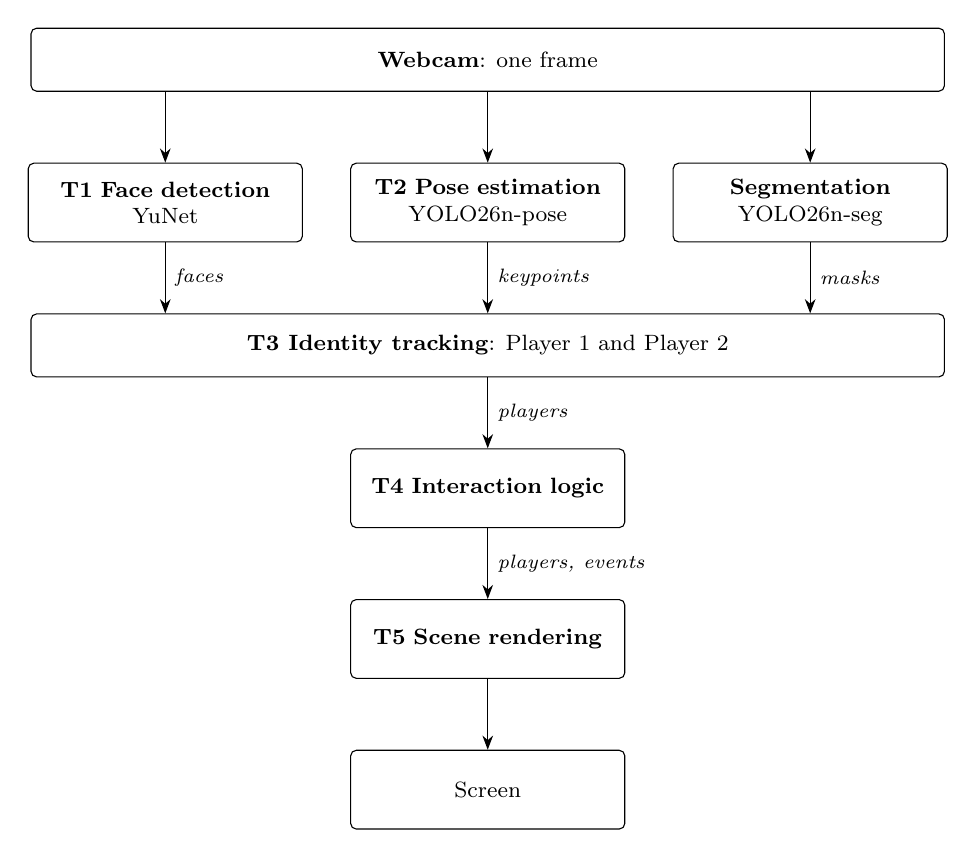
\begin{tikzpicture}[
      font=\footnotesize,
      >={Stealth[length=1.8mm]},
      node distance=9mm and 6mm,
      box/.style={draw, rounded corners=2pt, align=center, text width=3.2cm, inner sep=4pt, minimum height=10mm},
      wide/.style={draw, rounded corners=2pt, align=center, minimum width=11.6cm, inner sep=4pt, minimum height=8mm},
      lbl/.style={font=\scriptsize\itshape, right}]
    \node[box] (pose) {\textbf{T2 Pose estimation}\\ YOLO26n-pose};
    \node[box, left=of pose] (face) {\textbf{T1 Face detection}\\ YuNet};
    \node[box, right=of pose] (seg) {\textbf{Segmentation}\\ YOLO26n-seg};
    \node[wide, above=of pose] (cam) {\textbf{Webcam}: one frame};
    \node[wide, below=of pose] (id) {\textbf{T3 Identity tracking}: Player 1 and Player 2};
    \node[box, below=of id] (logic) {\textbf{T4 Interaction logic}};
    \node[box, below=of logic] (render) {\textbf{T5 Scene rendering}};
    \node[box, below=of render] (screen) {Screen};
    \draw[->] (cam.south -| face) -- (face);
    \draw[->] (cam.south -| pose) -- (pose);
    \draw[->] (cam.south -| seg) -- (seg);
    \draw[->] (face) -- node[lbl] {faces} (face |- id.north);
    \draw[->] (pose) -- node[lbl] {keypoints} (pose |- id.north);
    \draw[->] (seg) -- node[lbl] {masks} (seg |- id.north);
    \draw[->] (id) -- node[lbl] {players} (logic);
    \draw[->] (logic) -- node[lbl] {players, events} (render);
    \draw[->] (render) -- (screen);
  \end{tikzpicture}
\end{document}
